\documentclass{article}
\usepackage{graphicx}
\usepackage[left=3.5cm, right = 3.5cm, top=3.5cm, bottom=3.5cm, head=13.6pt]{geometry}
\usepackage[onehalfspacing]{setspace}
\usepackage{amsthm}
\usepackage{amsmath}
\usepackage{amssymb}
\usepackage{mathtools}
\usepackage{float}
\usepackage{algpseudocode}
\usepackage{algorithm}
\usepackage{comment}
\usepackage{csquotes}
\usepackage{enumitem}


\title{Advanced Topics in Computer Graphics I - Sheet R04}
\author{Ninian Kaspers, Robin Landsgesell, Julian Stamm}
\date{\today}

\begin{document}

    \maketitle

    \section*{Assignment 2}
    
    In the right image a Phong BRDF was used. The blur looks more uniform which corresponds to the simple formulation of the Phong BRDF using only the angle between the reflection vector and the view vector to determine the shape of the reflection.\\
    In the left image a micro-facet BRDF was used. It models effects appearing at grazing angles more accurately. At grazing angles the larger tail of the NDF for a rough surface causes the blur of the reflections look more directional. This comes from the amount of microfacets that still contribute at these angles even though the viewing angle differs significantly from the ideal reflection direction. If the NDF is based on the tangent of the normal and the half-vector, this tangent causes this slower falloff producing the longer tails. Furthermore, the Fresnel term causes the reflection at grazing angles to appear brighter and even though the geometric term decreases this effect the reflection in the left image still seems to be brighter.

    \section*{Assignment 3}

    \begin{enumerate}[label=\alph*)]
        \item 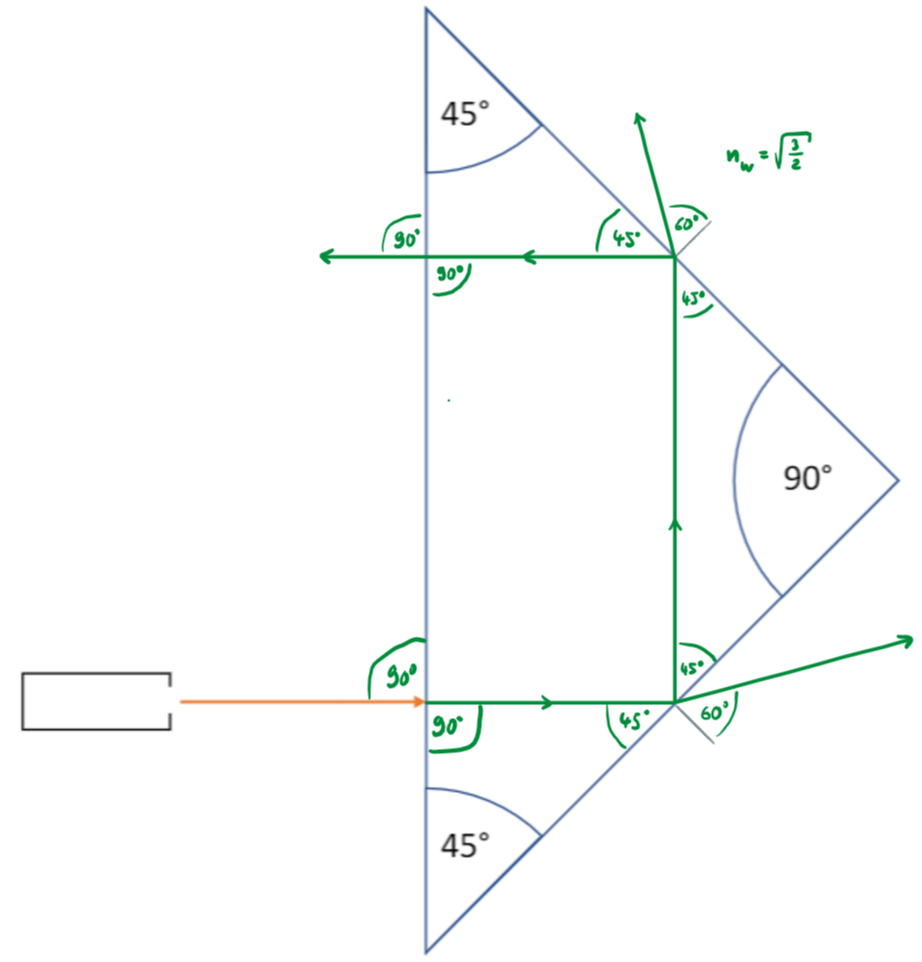
\includegraphics[width=0.5\textwidth]{3a.png}
        \item 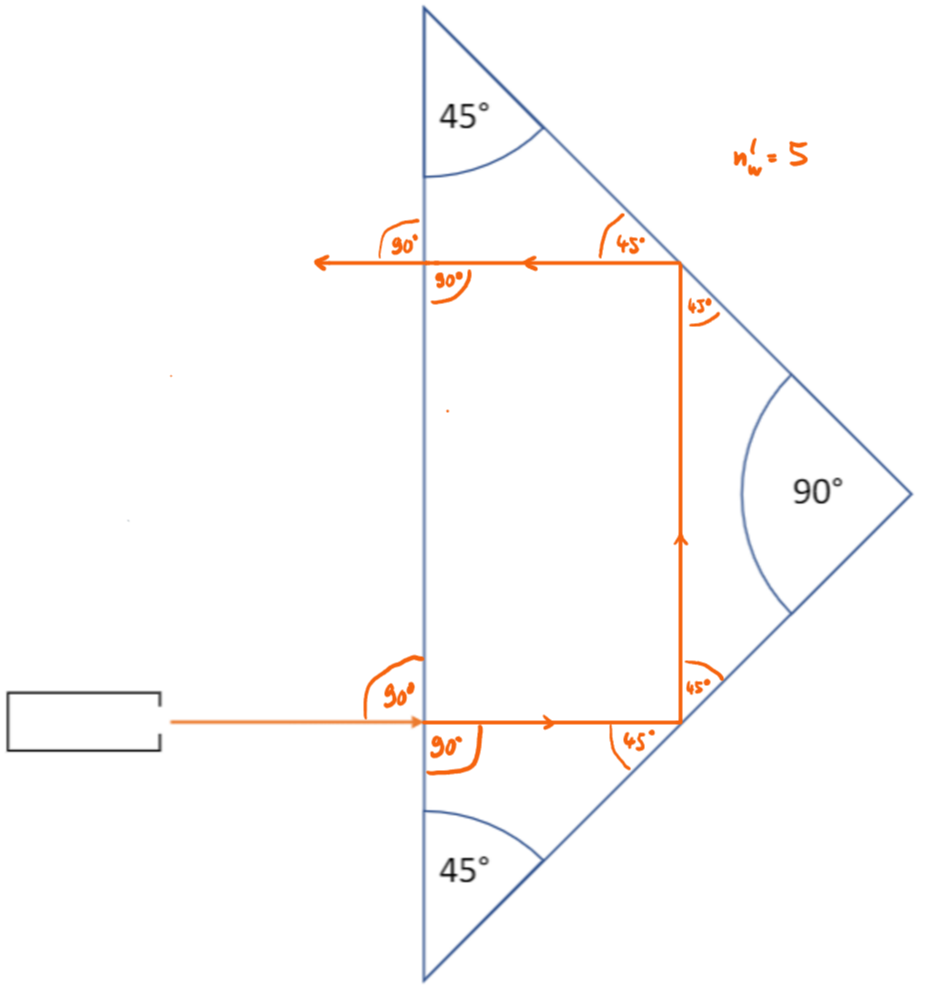
\includegraphics[width=0.5\textwidth]{3b.png}
        \item For b) the refractive index of the wedge was so high, that the light ray will not leave the wedge on the right side because of total internal reflection.
        \item $\hat{n}_w \sin(45^\circ) = n_a \sin(90^\circ) \Leftrightarrow \hat{n}_w = \sqrt{2}$ is the smallest refractive index leading to the same result.
    \end{enumerate}
    
\end{document}
